\chapter{Results \& Discussion}\label{ch:results}
The results and discussion for all tests regarding both the GAN and OCR are presented in this chapter. Both the qualitative and quantitative results are provided for the evaluation of GAN models as discussed in the previous chapter. The quantitative results of GAN are discussed using the bar plots with metrics such as SSIM, FID and MSE while the qualitative results are discussed using visual results of test images from the output of the GAN generator. Then character recognition is evaluated using both the google vision API and the proposed integrated OCR engine. This chapter is concluded with the discussion of the effectiveness of GAN in terms of improvement in the character detection and recognition of the steel type plate images.

\section{Results of GAN}
Both the quantitative and qualitative results regarding the steel type plate images translated by the GAN models are presented below.

\subsection{Quantitative results}
As discussed earlier in the previous chapter, the GAN models are evaluated using three different metrics: i) FID, ii) SSIM and iii) MSE. The bar chart (Figure \ref{fig:fid}) below gives information about how the test images are evaluated using the FID metric. Lower FID indicates the better quality of generated images. The results obtained from the FID evaluation showed that the pix2pix model does well among the other models. The results of pix2pix have the lowest FID score of 15.09  and outperform other models by a significant margin. The use of synthetic data produces similar kinds of results for the pix2pix model. The CycleGAN performs the worst with a score of 51.76. This can be explained by the fact that the model is trained in an unsupervised manner with fewer data points. The FactorGAN produced slightly better results compared to the CycleGAN with a score of 32.35, but not as good as pix2pix.

\begin{figure}[H]
\centering
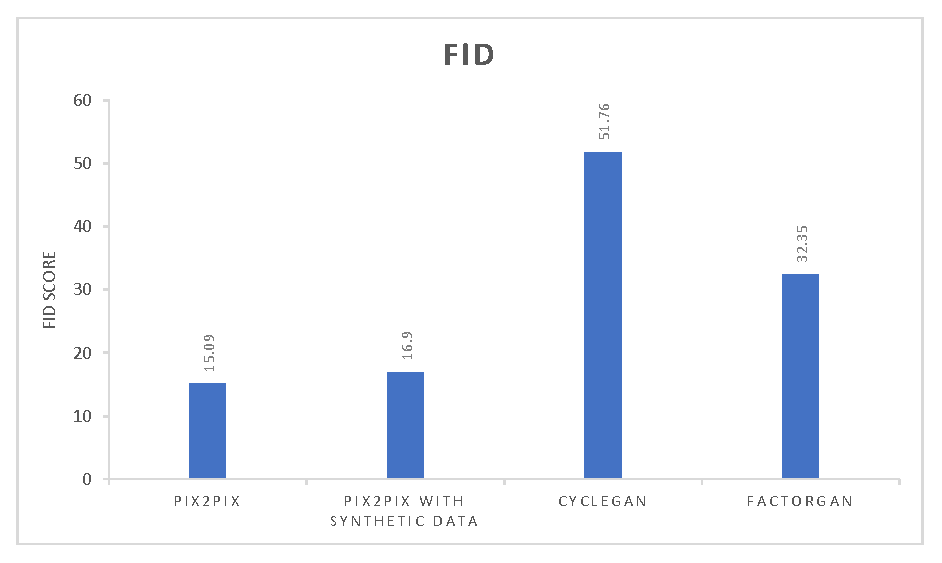
\includegraphics[width=4in]{images/FID.eps}
\caption{Experimental results for FID}
\label{fig:fid}
\end{figure}


In a search for a still more accurate result, the pix2pix model is trained with the synthetic dataset along with the real dataset. This also produced similar results as that of the pix2pix model trained only with the original image dataset. The difference between both the results were very minute as seen in the quantitative results and could not be differentiated during the qualitative evaluation. The CycleGAN and FactorGAN architecture have 4 networks each in total as discussed in Chapter \ref{ch:method}. The time taken for training both the models is very high in general. Also, they produced the worst results compared to the pix2pix while using the original dataset. Therefore the experiments with the synthetic dataset were not conducted for both CycleGAN and FactorGAN.  
\newline
	
	The SSIM score gives the similarity between ground truth data and the output of the generator for the test images. Higher SSIM indicates better quality of generated images. The chart shown in the Figure \ref{fig:ssim} shows the SSIM scores evaluated for different GAN models. The results of SSIM is exactly similar to the FID evaluation. The model that has the best SSIM score is pix2pix with a similarity score of 0.8. The model trained with synthetic dataset + pix2pix produces similar results that of pix2pix with a score of 0.79. The SSIM score for FactorGAN and CycleGAN is very low compared to other models with a score of 0.74 and 0.69 respectively.

\begin{figure}[H]
\centering
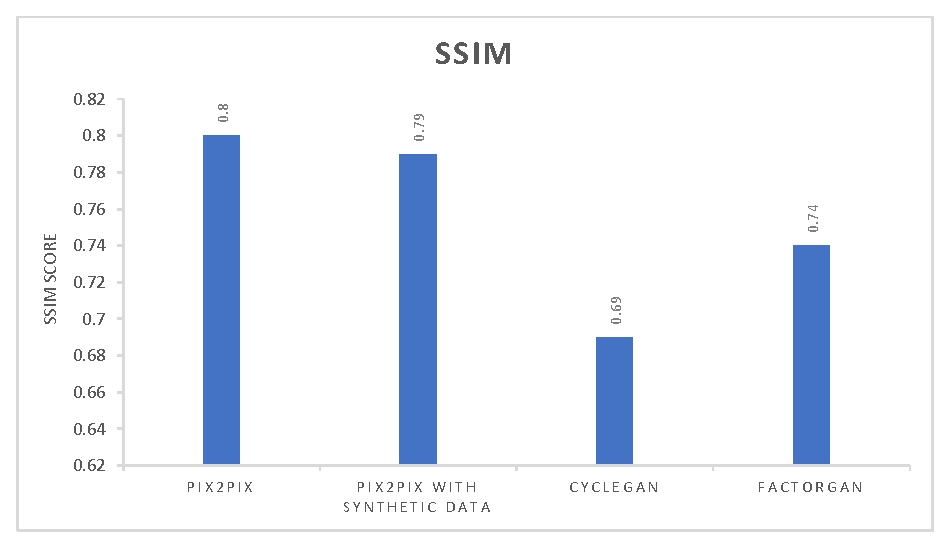
\includegraphics[width=4in]{images/ssim.eps}
\caption{Experimental results for SSIM}
\label{fig:ssim}
\end{figure}

	The MSE is calculated by squaring the absolute difference between the pixels of ground truth and the generated image. The result of this experiment is shown in Figure \ref{fig:mse}. It is seen that the model trained with synthetic data with pix2pix GAN has the least error whereas the CycleGAN model with a MSE of 5739.08 performs the worst. The MSE for pix2pix does not differ much from the best model with the value of 3377.56 while the MSE of FactorGAN is 3664.83.

\begin{figure}[H]
\centering
\includegraphics[width=4in]{images/mse.eps}
\caption{Experimental results for MSE}
\label{fig:mse}
\end{figure}

\subsection{Qualitative results}
The qualitative results are evaluated by manual visual inspection of translated test images for all three different GANs. Figures \ref{test1} - \ref{test3} show how different models perform when translating the image from unclear to a clearer image. Since it is not possible to display all the images, we have shown the test results of three sample images with their ground truth and corresponding translation by three different GANs. 
\newline	

	
	Both the quantitative and qualitative results of the experiment can be found in the GitLab link shared in Section \ref{sec:imp}.  It can also be accessed using the shared google drive \url{https://drive.google.com/drive/folders/1lMbM0bjMx1LoIyi8cyV7Nz1Gy5yUisXB?usp=sharing}. The qualitative results support the findings of the quantitative results. From the results, it can be seen that the pix2pix model successfully generate images very close to ground truth images. The use of ResNet as a feature extractor combined with paired dataset and techniques such as random cropping of the input image to the size of 256 x 256 for each epoch during training contributed to the success of the pix2pix model. This complements the experiments for quantitative evaluation. The misclassified characters for pix2pix are mostly repetitive. In rare cases, the texts were incorrectly transformed or missed. For example, the characters such as 'D', '/', 'G' in the steel plates are misclassified as '0', '7', '6' respectively.
\newline	
	
		
\begin{figure}[H]
\begin{tabular}{cc}
\includegraphics[width=65mm]{images/i2.jpg} &   \includegraphics[width=65mm]{images/g2.jpg} \\
(a) Input & (b) Ground Truth \\[6pt]
 \includegraphics[width=65mm]{images/p2.jpg} &   \includegraphics[width=65mm]{images/c2.jpg} \\
(c) Pix2pix & (d) CycleGAN \\[6pt]
\multicolumn{2}{c}{\includegraphics[width=65mm]{images/f2.jpg} }\\
\multicolumn{2}{c}{(e) FactorGAN}
\end{tabular}
\caption{Test result: Sample 1}
\label{test1}
\end{figure}

The CycleGAN produces the worst results though it uses ResNet as a feature extractor. From Figures \ref{test1} - \ref{test3}, it can be seen that CycleGAN misses a lot of text areas compared to the annotated images. It gives decent output only when the text area is clear in the original image. It fails to segment the characters when the corresponding area in the input image has even a little bit of noise such as reflection or under different lighting conditions.  Thus CycleGAN skips a lot of characters and could not translate the complete structure of the input image. Thus it results in huge MSE loss, worst SSIM
\begin{figure}[H]
\begin{tabular}{cc}
\includegraphics[width=65mm]{images/i1.jpg} &   \includegraphics[width=65mm]{images/g1.jpg} \\
(a) Input & (b) Ground Truth \\[6pt]
 \includegraphics[width=65mm]{images/p1.jpg} &   \includegraphics[width=65mm]{images/c1.jpg} \\
(c) Pix2pix & (d) CycleGAN \\[6pt]
\multicolumn{2}{c}{\includegraphics[width=65mm]{images/f1.jpg} }\\
\multicolumn{2}{c}{(e) FactorGAN}
\end{tabular}
\caption{Test result: Sample 2}
\label{test2}
\end{figure}
\noindent
and FID score as found during the quantitative evaluation. The use of unsupervised learning, unpaired dataset and insufficient data points are the probable reasons for the failure of CycleGAN.
\newline	

	
\begin{figure}[H]
\begin{tabular}{cc}
\includegraphics[width=65mm]{images/i4.jpg} &   \includegraphics[width=65mm]{images/g4.jpg} \\
(a) Input & (b) Ground Truth \\[6pt]
 \includegraphics[width=65mm]{images/p4.jpg} &   \includegraphics[width=65mm]{images/c4.jpg} \\
(c) Pix2pix & (d) CycleGAN \\[6pt]
\multicolumn{2}{c}{\includegraphics[width=65mm]{images/f4.jpg} }\\
\multicolumn{2}{c}{(e) FactorGAN}
\end{tabular}
\caption{Test result: Sample 3}
\label{test3}
\end{figure}

The much expected FactorGAN did not live up to its expectations either. Even though \citeauthor{stoller2019training}'s hypothesis of improved segmentation accuracy over CycleGAN still holds true for our experiments with steel type plates dataset, the pix2pix GAN produces results which are far better from the results of FactorGAN. This may be because our dataset is very different from the cityscapes dataset \citep{cordts2016cityscapes} that was used in the \citeauthor{stoller2019training} experiments for training FactorGAN. The classes of cityscapes dataset fall under seven groups like human, vehicle, construction, etc,. Their classes have a broader boundary and include large objects whereas our steel type plate dataset mainly consists of two classes: characters and background which have a finer class boundary. The results of FactorGAN show that it captures all the necessary character segmentation areas like pix2pix but the translations are very blurry and cannot be used for character recognition. Thus the FactorGAN has only the second-best results during the quantitative evaluation. 
\newline

	In general, the translation becomes problematic when the font size of the text present in the images is very small or very big. Also, it was noted in the results that embossed texts were not correctly transformed in many test cases. This can be due to the fact that the images in our dataset had more samples of engraved texts than embossed texts. 
\newline
	
	From both the quantitative and qualitative evaluation, the pix2pix model stands out as the best model. So the final proposed framework consists of a pix2pix model for translating the noisy steel plates to clear images. 
	
\section{Results of OCR}
For evaluating the efficiency of the use of GAN for character recognition, we randomly cropped the 30 test images to the size 256 x 256 and translated it using pix2pix GAN. Both the original image and its GAN translated image is passed into the OCR engine for character recognition. In this thesis we experimented with two different OCR engines: i) The commercial OCR engine using Google Vision API ii) The proposed CRAFT based OCR engine. The results of the experiments are tabulated in Tables \ref{tab:ocrtab1} - \ref{tab:ocrtab3}.				

\subsection{Evaluation using Google Vision OCR}
	Table \ref{tab:ocrtab1} compares the character recognition before and after the use of the GAN translated image using Google Vision OCR. The table presents the total number of characters present in the test images, the number of characters recognized by the Google Vision OCR engine and the average OCR Score. The number of characters recognized is further split into characters correctly identified, incorrectly identified and missed.

\begin{table}[H]
\resizebox{\textwidth}{!}{%
\begin{tabular}{@{}|c|c|c|c|c|c|c|@{}}
\toprule
 &
  \textbf{\begin{tabular}[c]{@{}c@{}}Total number of \\ characters\end{tabular}} &
  \textbf{\begin{tabular}[c]{@{}c@{}}Characters \\ recognized\end{tabular}} &
  \textbf{\begin{tabular}[c]{@{}c@{}}Correctly \\ identified\end{tabular}} &
  \textbf{\begin{tabular}[c]{@{}c@{}}Incorrectly \\ identified\end{tabular}} &
  \textbf{\begin{tabular}[c]{@{}c@{}}Characters \\ missed\end{tabular}} &
  \textbf{OCR Score} \\ \midrule
\textbf{\begin{tabular}[c]{@{}c@{}}Character recognition\\  without GAN\end{tabular}} &
  1303 &
  1054 &
  914 &
  140 &
  249 &
  67.06 \\ \midrule
\textbf{\begin{tabular}[c]{@{}c@{}}Character recognition \\ with GAN\end{tabular}} &
  1303 &
  1287 &
  1104 &
  183 &
  16 &
  84.09 \\ \bottomrule
\end{tabular}%
}
\caption{Character recognition with and without GAN using Google Vision OCR engine}
\label{tab:ocrtab1}
\end{table}

\begin{figure}[H]
\centering
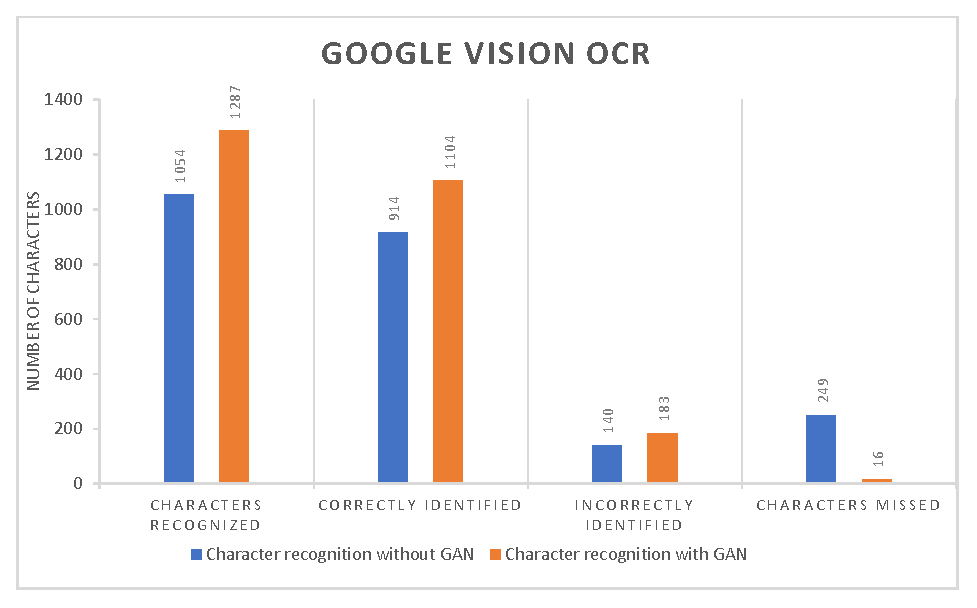
\includegraphics[width=5in]{images/ocrcomp3.eps}
\caption{Evaluation of character recognition using Google Vision}
\label{fig:ocrcomp3}
\end{figure}

 The total number of characters present in the test images is 1303. The total number of characters recognized for original images is 1054 whereas the total number of characters recognized significantly increased to 1287 when using their corresponding GAN translated images. Also, the characters missed are drastically reduced from 249 to 16 when using GAN translated images. The results in the above table are plotted using a bar chart in Figure \ref{fig:ocrcomp3}.



\subsection{Evaluation using the proposed OCR}


The same experiment is repeated for the proposed OCR engine with the same test images for evaluating the efficiency of the use of GAN in character recognition. The results are tabulated in Table \ref{tab:ocrtab2}. It compares the character recognition before and after the use of GAN translated image using the proposed OCR. Similar to Table \ref{tab:ocrtab1}, this table presents the total number of characters present in the test images, the number of characters recognized by the proposed OCR engine and its average OCR score.
\begin{table}[H]
\resizebox{\textwidth}{!}{%
\begin{tabular}{@{}|c|c|c|c|c|c|c|@{}}
\toprule
 &
  \textbf{\begin{tabular}[c]{@{}c@{}}Total number of \\ characters\end{tabular}} &
  \textbf{\begin{tabular}[c]{@{}c@{}}Characters \\ recognized\end{tabular}} &
  \textbf{\begin{tabular}[c]{@{}c@{}}Correctly \\ identified\end{tabular}} &
  \textbf{\begin{tabular}[c]{@{}c@{}}Incorrectly \\ identified\end{tabular}} &
  \textbf{\begin{tabular}[c]{@{}c@{}}Characters\\  missed\end{tabular}} &
  \textbf{OCR score} \\ \midrule
\textbf{\begin{tabular}[c]{@{}c@{}}Character recognition \\ without GAN\end{tabular}} &
  1303 &
  1036 &
  830 &
  206 &
  267 &
  61.78 \\ \midrule
\textbf{\begin{tabular}[c]{@{}c@{}}Character recognition\\  with GAN\end{tabular}} &
  1303 &
  1267 &
  1094 &
  173 &
  36 &
  84.37 \\ \bottomrule
\end{tabular}%
}
\caption{Character recognition with and without GAN using the proposed OCR engine}
\label{tab:ocrtab2}
\end{table}

In case of proposed OCR, the character recognition is increased from 1036 to 1267 when using GAN translated images. Also, the characters missed are reduced from 267 to 36 when using GAN translated images. The results in the above table are plotted using a bar chart in Figure \ref{fig:ocrcomp3}.

	
\begin{figure}[H]
\centering
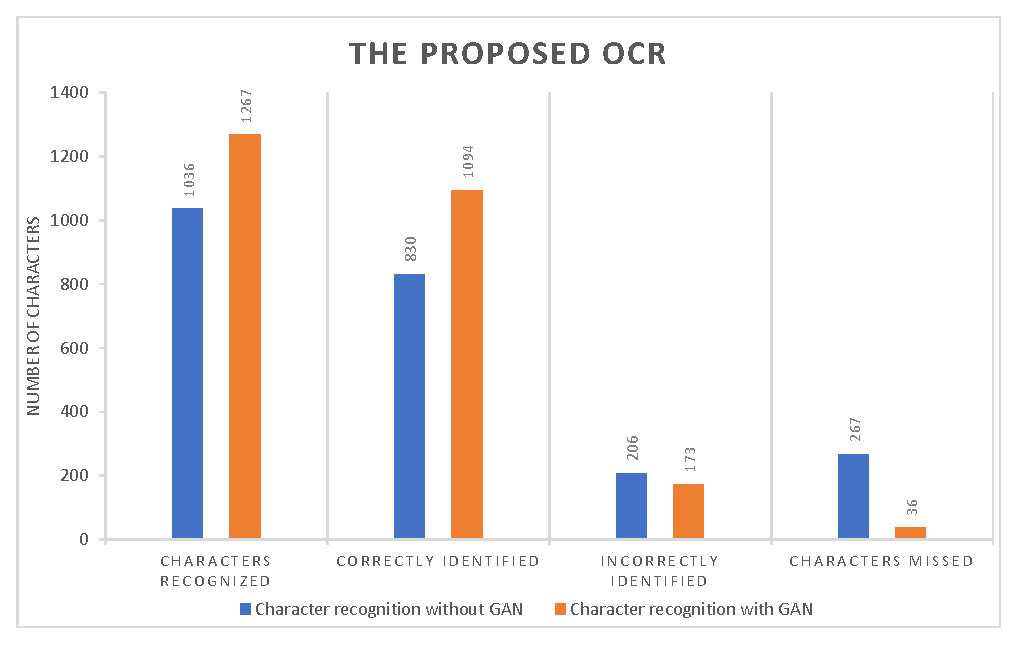
\includegraphics[width=5in]{images/ocrcomp4.eps}
\caption{Evaluation of character recognition using the proposed OCR engine}
\label{fig:ocrcomp4}
\end{figure}

Tables \ref{tab:ocrtab1} and \ref{tab:ocrtab2} show that the average OCR score for Google Vision OCR is increased from 67.06 \% to 84.09 \% while the average OCR score is massively increased from 61.78 \% to 84.37 \% when using the GAN translated image.

\subsection{Comparison of OCR engines}
This section compares the impact of image-to-image translation GAN on both the OCR engine in terms of improvement of character recognition. Table \ref{tab:ocrtab3} presents the comparison of both the OCR engines in terms of improvement in character recognition when using GAN. 
\newline

	As discussed above in the tables \ref{tab:ocrtab1} \& \ref{tab:ocrtab2}, when using GAN translated image, the character recognition i.e. the detection of the number of characters in the steel type plates is improved by 20.09 \% for the proposed OCR. Even for the commercial OCR tool like Google Vision, the character recognition of steel type plates is improved by 20.16 \%. 
\begin{table}[H]
\resizebox{\textwidth}{!}{%
\begin{tabular}{@{}|c|c|c|@{}}
\toprule
\textbf{OCR engine} &
  \textbf{\begin{tabular}[c]{@{}c@{}}Improvement of character \\ recognition using GAN \\ translated Image\end{tabular}} &
  \textbf{\begin{tabular}[c]{@{}c@{}}Percentage increase\\  in OCR Score\end{tabular}} \\ \midrule
\textbf{The proposed OCR} &
  20.09 &
  36.57 \\ \midrule
\textbf{Google Vision} &
  20.16 &
  25.39 \\ \bottomrule
\end{tabular}%
}
\caption{Comparison of impact of GAN on both OCR engines}
\label{tab:ocrtab3}
\end{table}

Similarly, the OCR score for Google Vision is improved by 25.39 \% while for the proposed OCR, it has been massively increased by 36.57 \%. This is graphically represented using a bar chart in Figure \ref{fig:ocrcomp5}.


\begin{figure}[H]
\centering
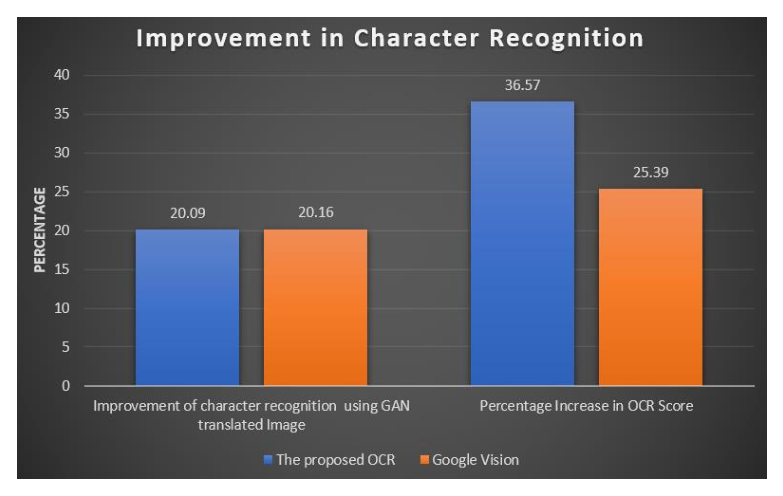
\includegraphics[width=5in]{images/ocrcomp5.eps}
\caption{Comparison of impact of GAN on both OCR engines}
\label{fig:ocrcomp5}
\end{figure}